\clearpage
\section{Systematic uncertainties}
\label{sec:systematic-uncertainties}

In an experimental analysis, most if not all of the measured and predicted observables have uncertainties associated with them. These uncertainties can be experimental in nature, such as an uncertainty on the reconstruction efficiency of the muons in the detector, or theoretical, such as an uncertainty on a cross section. As a general rule, an uncertainty that scales with the number of events is referred to as statistical, while one that cannot be reduced by increasing the statistics is referred to as a systematic uncertainty. It could well be that a statistical uncertainty in one study becomes a systematic uncertainty in another.

As mentioned, there are uncertainties associated with theoretical calculations and simulation mismodeling (both for \FASTSIM and \FULLSIM), among other factors. This analysis follows all the recommendations listed by the \gls{cms} \gls{susy} \gls{pag}~\cite{sus-pag-recommendations}, which includes the study of muon scale factors described in Section~\ref{sec:scale-factors}. In this section, only the systematic uncertainties that are unique to this analysis are introduced, aside from the muon scale factors. The systematic uncertainties in this analysis are primarily due to the background estimation methods used.

\subsection{Data driven transfer factors}
\label{sec:data-driven-tranfer-factors}

Data-driven background estimations are used in both the dimuon category, to estimate the jetty non-isolated background, and in the exclusive track background. They involve computing a transfer factor in a dedicated \gls{cr} of $\text{BDT}<0$ and applying it in the \glspl{sr}. The transfer factors are computed as the ratio between the data counts in the main band and the sideband. In the dimuon category, the sideband is the isolation sideband, as described in Section~\ref{sec:jetty-background-estimation}, and for the exclusive track category, the sideband is the same-charge sideband, as described in Section~\ref{sec:ex-track-background-estimation}. These transfer factors have an associated uncertainty due to the statistics in the \gls{cr}. Table~\ref{tab:transfer-factors} lists all transfer factors and their associated uncertainties.

\begin{table}[hp]
	\centering
	\label{tab:transfer-factors}
		\caption{Transfer factors and their associated uncertainties}
		%\vspace{1mm}
			\begin{tabular}{lccccc} \hline
			Method & Flavor & Phase & Transfer Factor & Uncertainty & Relative Error \\ \hline
			Jetty & Muons & 0 &  0.548 & 0.078 & 14.2\% \\
			Jetty & Muons & 1 &  0.533 & 0.039 & 7.3\% \\
			\tautau & Muons & 0 &  0.518 & 0.411 & 79\% \\
			\tautau & Muons & 1 &  0.283 & 0.26 & 91.8\% \\
			Exclusive Track & Muons & 0 & 1.12 & 0.044 & 3.9\% \\ 
			Exclusive Track & Muons & 1 & 1.066 & 0.024 & 2.2\% \\	
			Exclusive Track & Electrons & 0 & 1.037 & 0.05 & 4.8\% \\	
			Exclusive Track & Electrons & 1 & 1.049 & 0.03 & 2.8\% \\			
			
			\hline
			\end{tabular}
\end{table}

\subsection{Data driven shape uncertainties}
\label{sec:data-driven-shape}

In the section about the background estimation methods, it is explained that the data-driven methods rely on the assumption that the shape of the background in a sideband is the same as in the main band and, therefore, require only a normalization factor to correctly predict the background. The exclusive track category closure plots in Figure~\ref{fig:ex-track-closure-tests} show no trend, and neither does the Phase 1 closure plot of the jetty background in Figure~\ref{fig:dimuon-bdt-jetty-2017-closure}. This is also supported by the line fit performed in the ratio panel, which is statistically consistent with a flat line intersecting 1.

In the dimuon category, only one \gls{bdt} is trained using 2017 simulation, but evaluated for phase 0 (2016) as well. This introduces a slight trend when a line is fit in the ratio panel of the closure plot in Figure~\ref{fig:dimuon-bdt-jetty-2016-closure}. The line fit is then used to introduce weights that are applied in an event-by-event manner with the value of the line for the specific \gls{bdt} value of the event. On the right side of Figure~\ref{fig:dimuon-bdt-jetty-2016-closure}, one can see the closure plot after said weights have been applied, and it is clear that the trend has been successfully eliminated.


\begin{figure}[!htb]
\centering
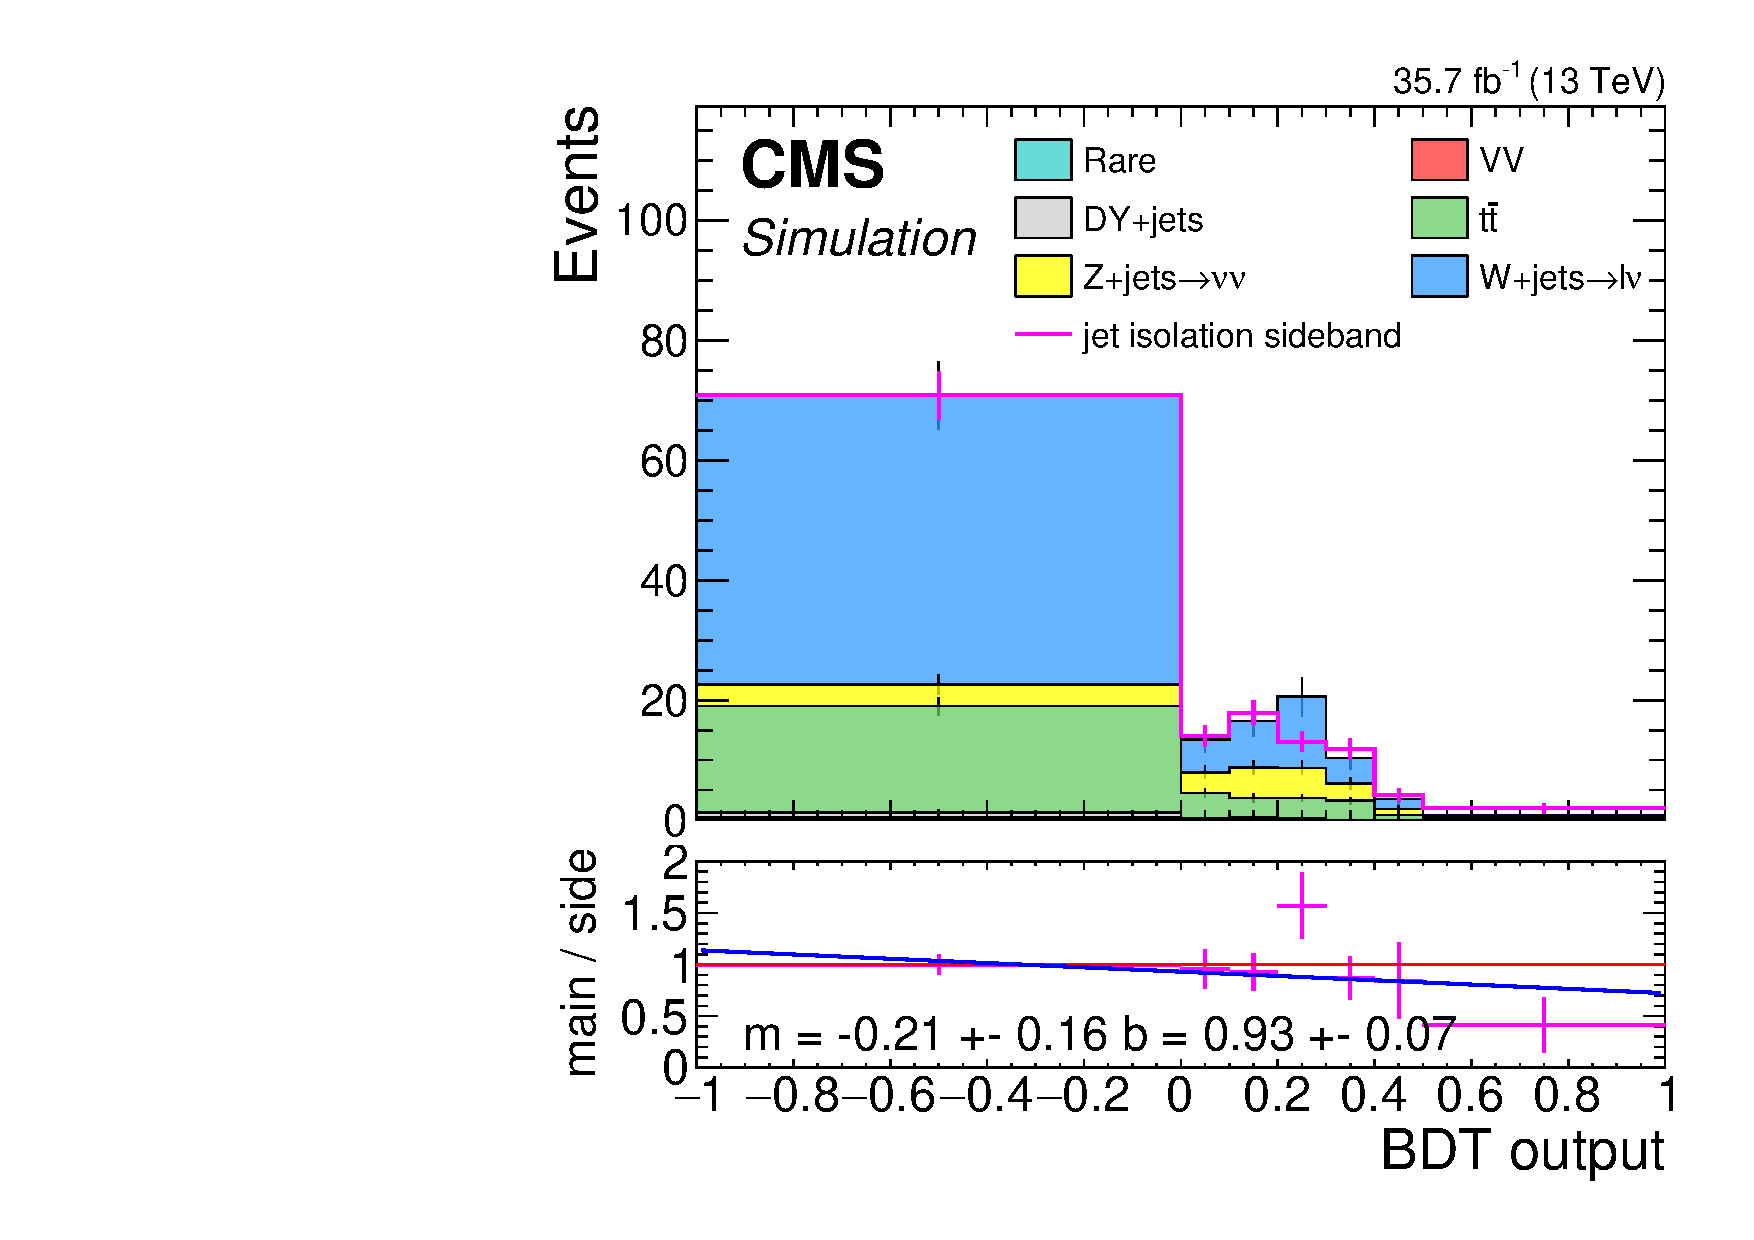
\includegraphics[width=0.48\linewidth]{plots/dilepton_muons_bg_isocr_no_retag_CorrJetNoMultIso10_06_2016_no_norm_sf/none_closure_dilepBDTphase1CorrJetNoMultIso10Dr0.6.pdf} \,
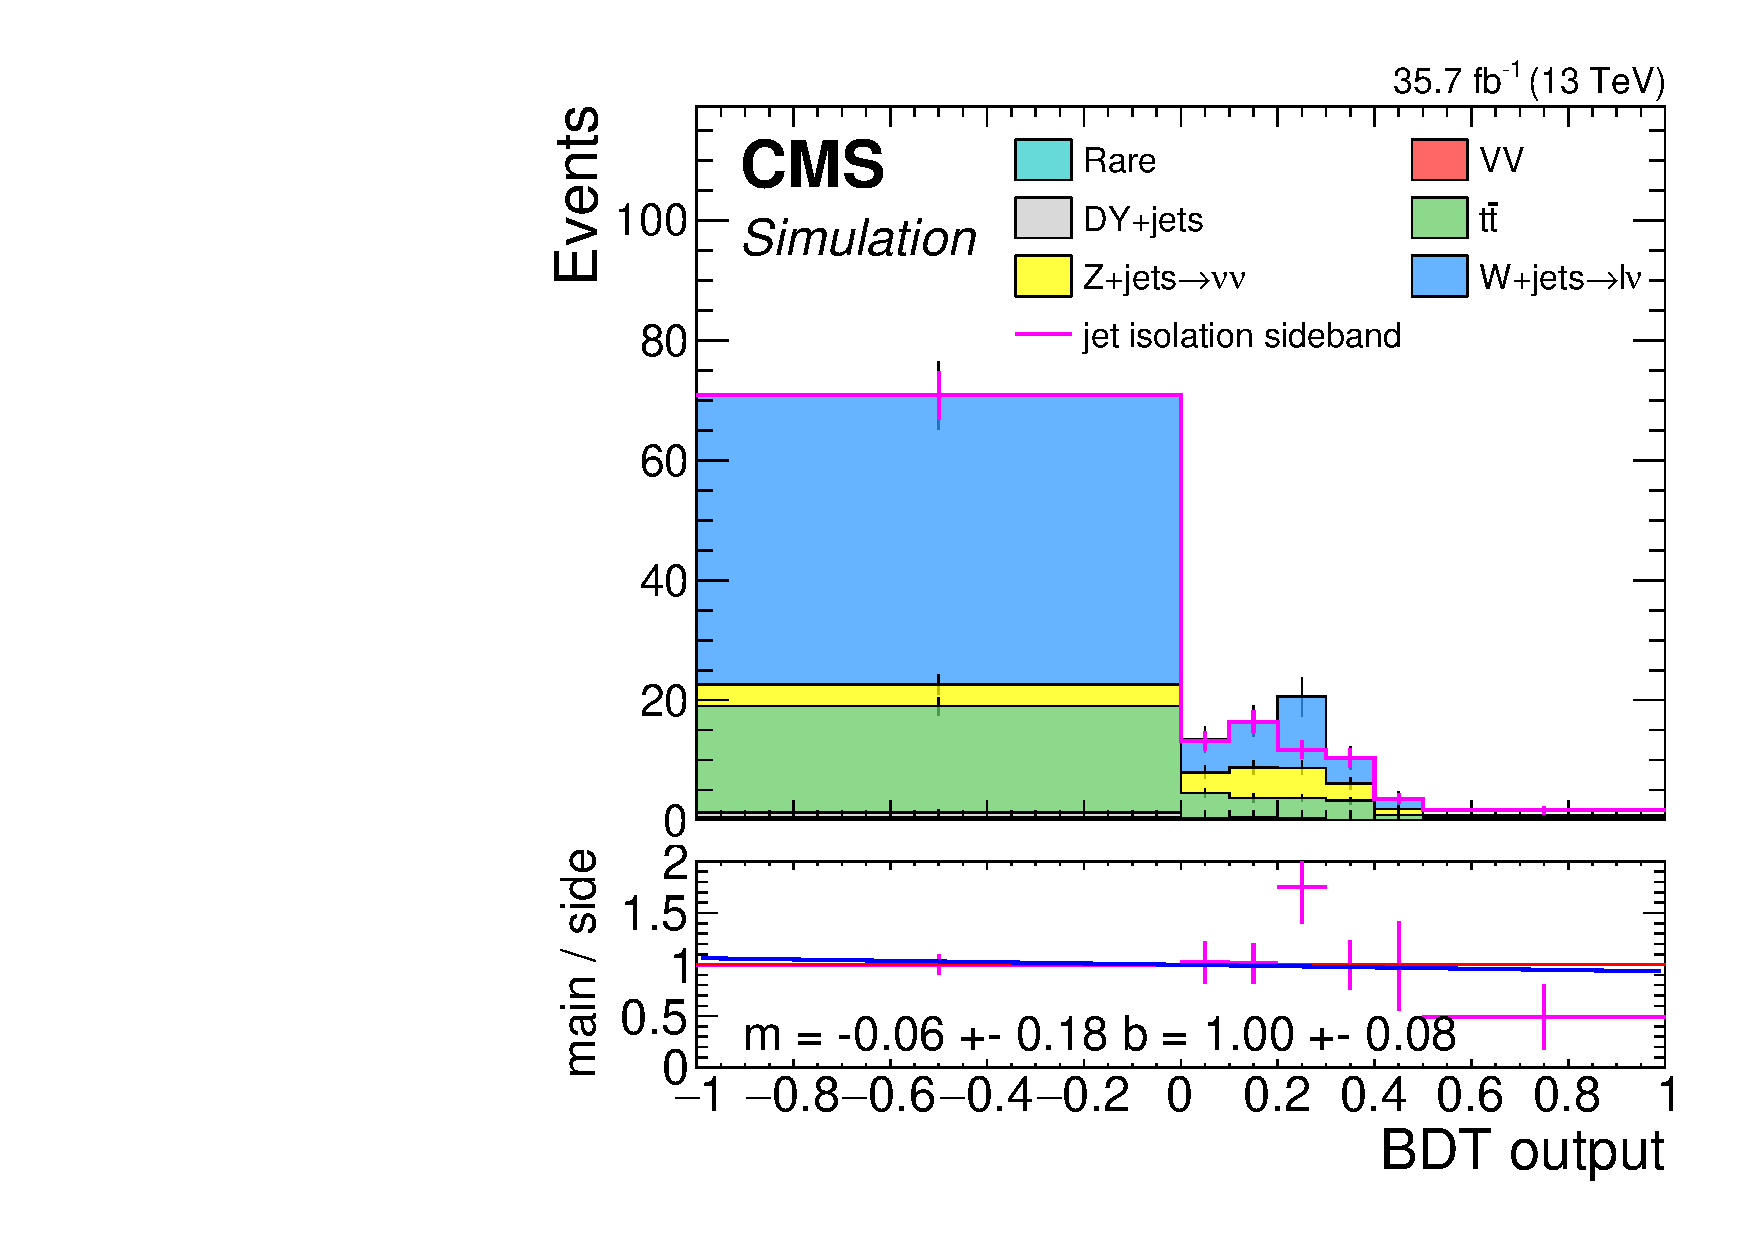
\includegraphics[width=0.48\linewidth]{plots/dilepton_muons_bg_isocr_no_retag_CorrJetNoMultIso10_06_2016_no_norm_sf_line_fit_line_weights/none_closure_dilepBDTphase1CorrJetNoMultIso10Dr0.6.pdf} 
 \\

\caption[Dimuon 2016 jetty background closure plots with and without fit line weights]{Dimuon 2016 jetty background closure plot with (right) and without (left) fit line weights. The stack represents simulation in the main isolation band after \ztautau has been removed, while the pink line represents simulation in the isolation sideband. The isolation sideband is normalized to match the isolation in the CR of $\mathrm{BDT} < 0$. The ratio panel shows the ratio between the isolatoin main band and sideband. A line fit of the ratio is performed and the parameters of the slope $m$ and interception point $b$ with their respective errors are stamped. In the plot on the right, the line fit weights obtained from the fit on the left plot have been applied.}
\label{fig:dimuon-bdt-jetty-2016-closure}
\end{figure}

On top of the transfer factor uncertainties listed in Table~\ref{tab:transfer-factors}, shape uncertainties taken from the line fits are also taken into account. For phase 1, since the closure plot line fit did not show any trend, the nominal values are taken without applying the line weights. For 2016, the nominal values are taken after the line weights were applied, i.e., from the right plot in Figure~\ref{fig:dimuon-bdt-jetty-2016-closure}. The alternative prediction, which is fed into the combine tool as the shape systematic uncertainty, is for 2017 the histogram with the line weights applied, and for 2016, since the weights were already applied as the nominal value, the weights of the fit line with the slope varied by $1\sigma$ are applied ($m=-0.21-0.16=-0.37$).


\subsection{Simulated background uncertainties}
\label{simulated-background-uncertainties}

The last background estimation method to consider is the \tautau background estimation, which uses simulation normalized to data in a \gls{cr}, as explained in Section~\ref{sec:mtautau-background-estimation}. For background methods that use simulation rather than data, normally a list of uncertainties associated with simulation uncertainties have to be applied. However, as could be seen in Figure~\ref{fig:data-driven-full-background-prediction}, this background is non-existent in the most sensitive bin, and is very small in the rest of the bins. Therefore, the already very large uncertainties on this background (79\%-92\%) are dominant enough that all other uncertainties can be safely neglected.

\begin{figure}[!htb]
\centering
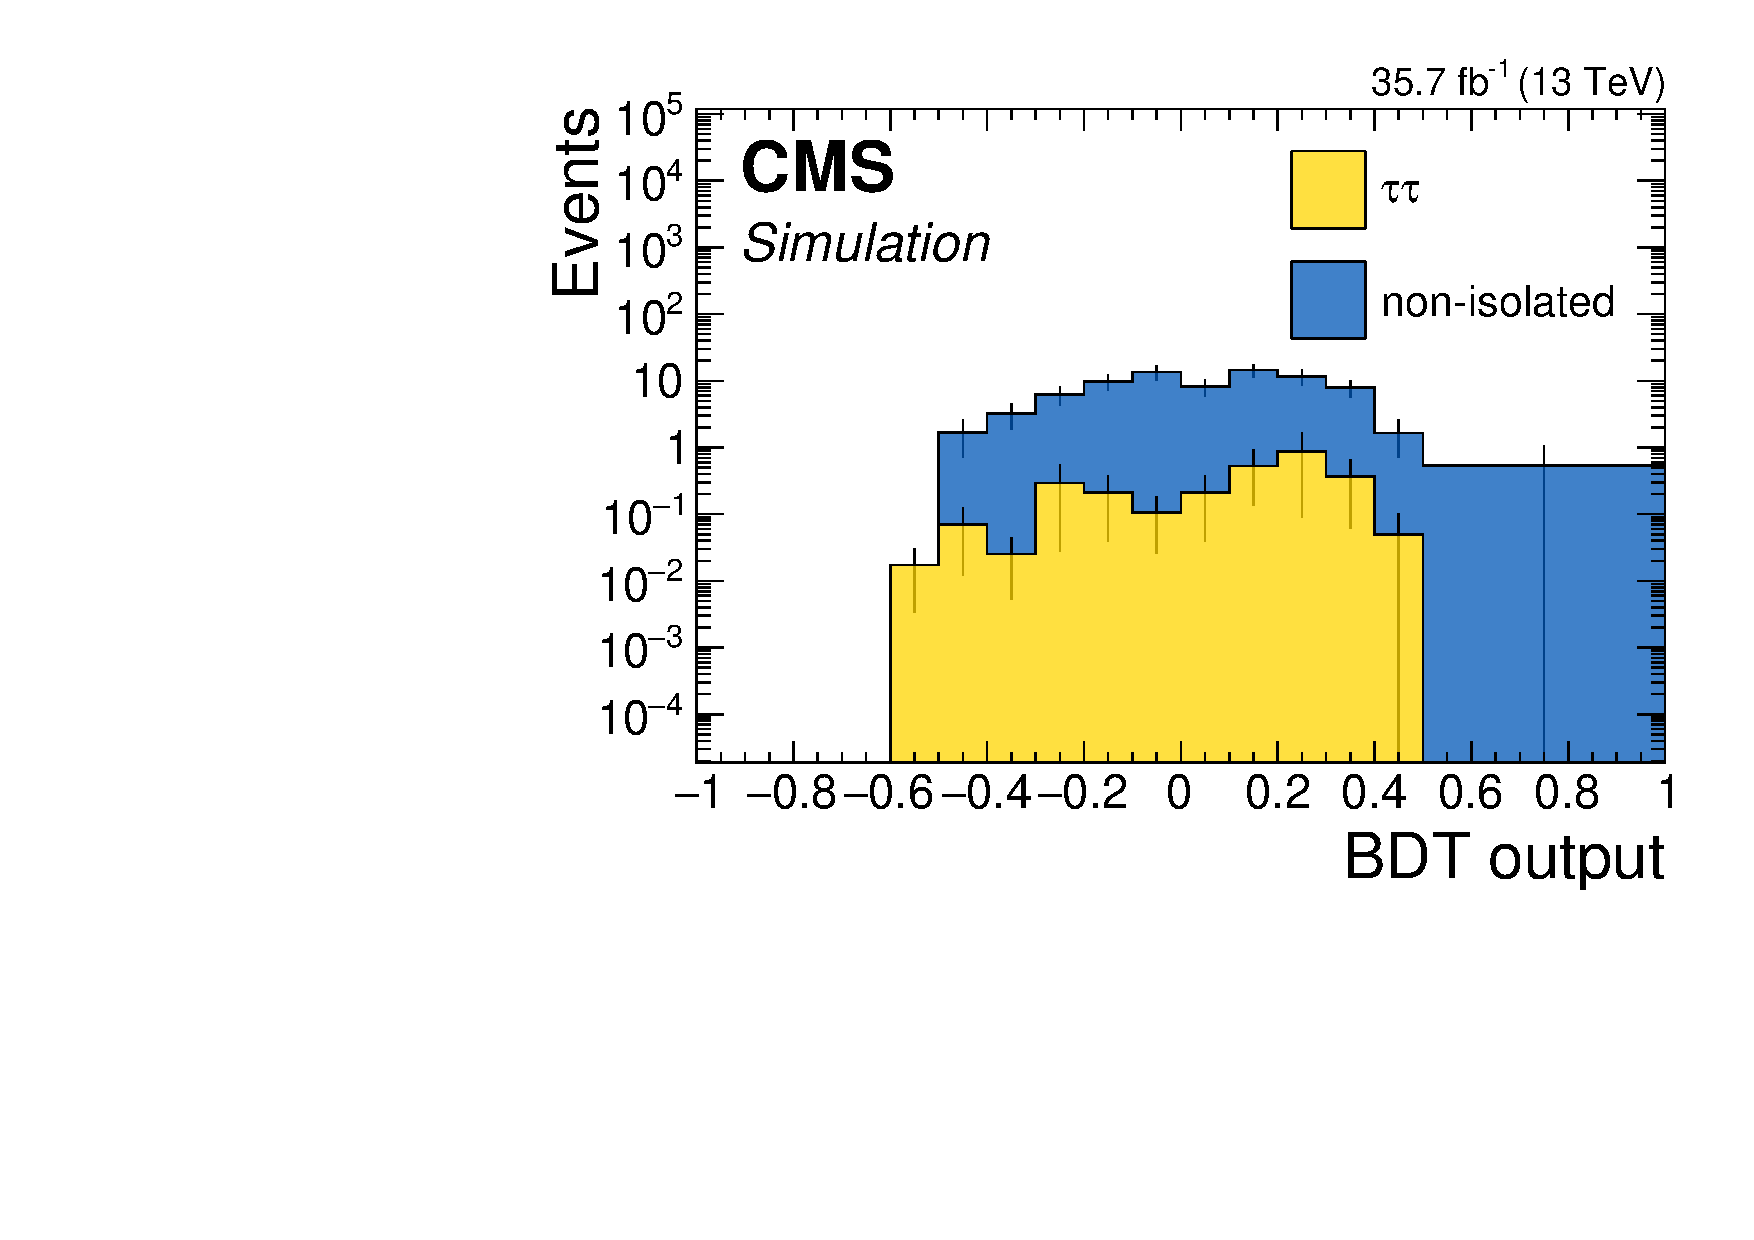
\includegraphics[width=0.48\linewidth]{plots/dimuon_background_estimation_non_isolated_and_tautau_2016/orth-notautau1_newestestest_bin_dilepBDTphase1CorrJetNoMultIso10Dr0.6_log.pdf} \,
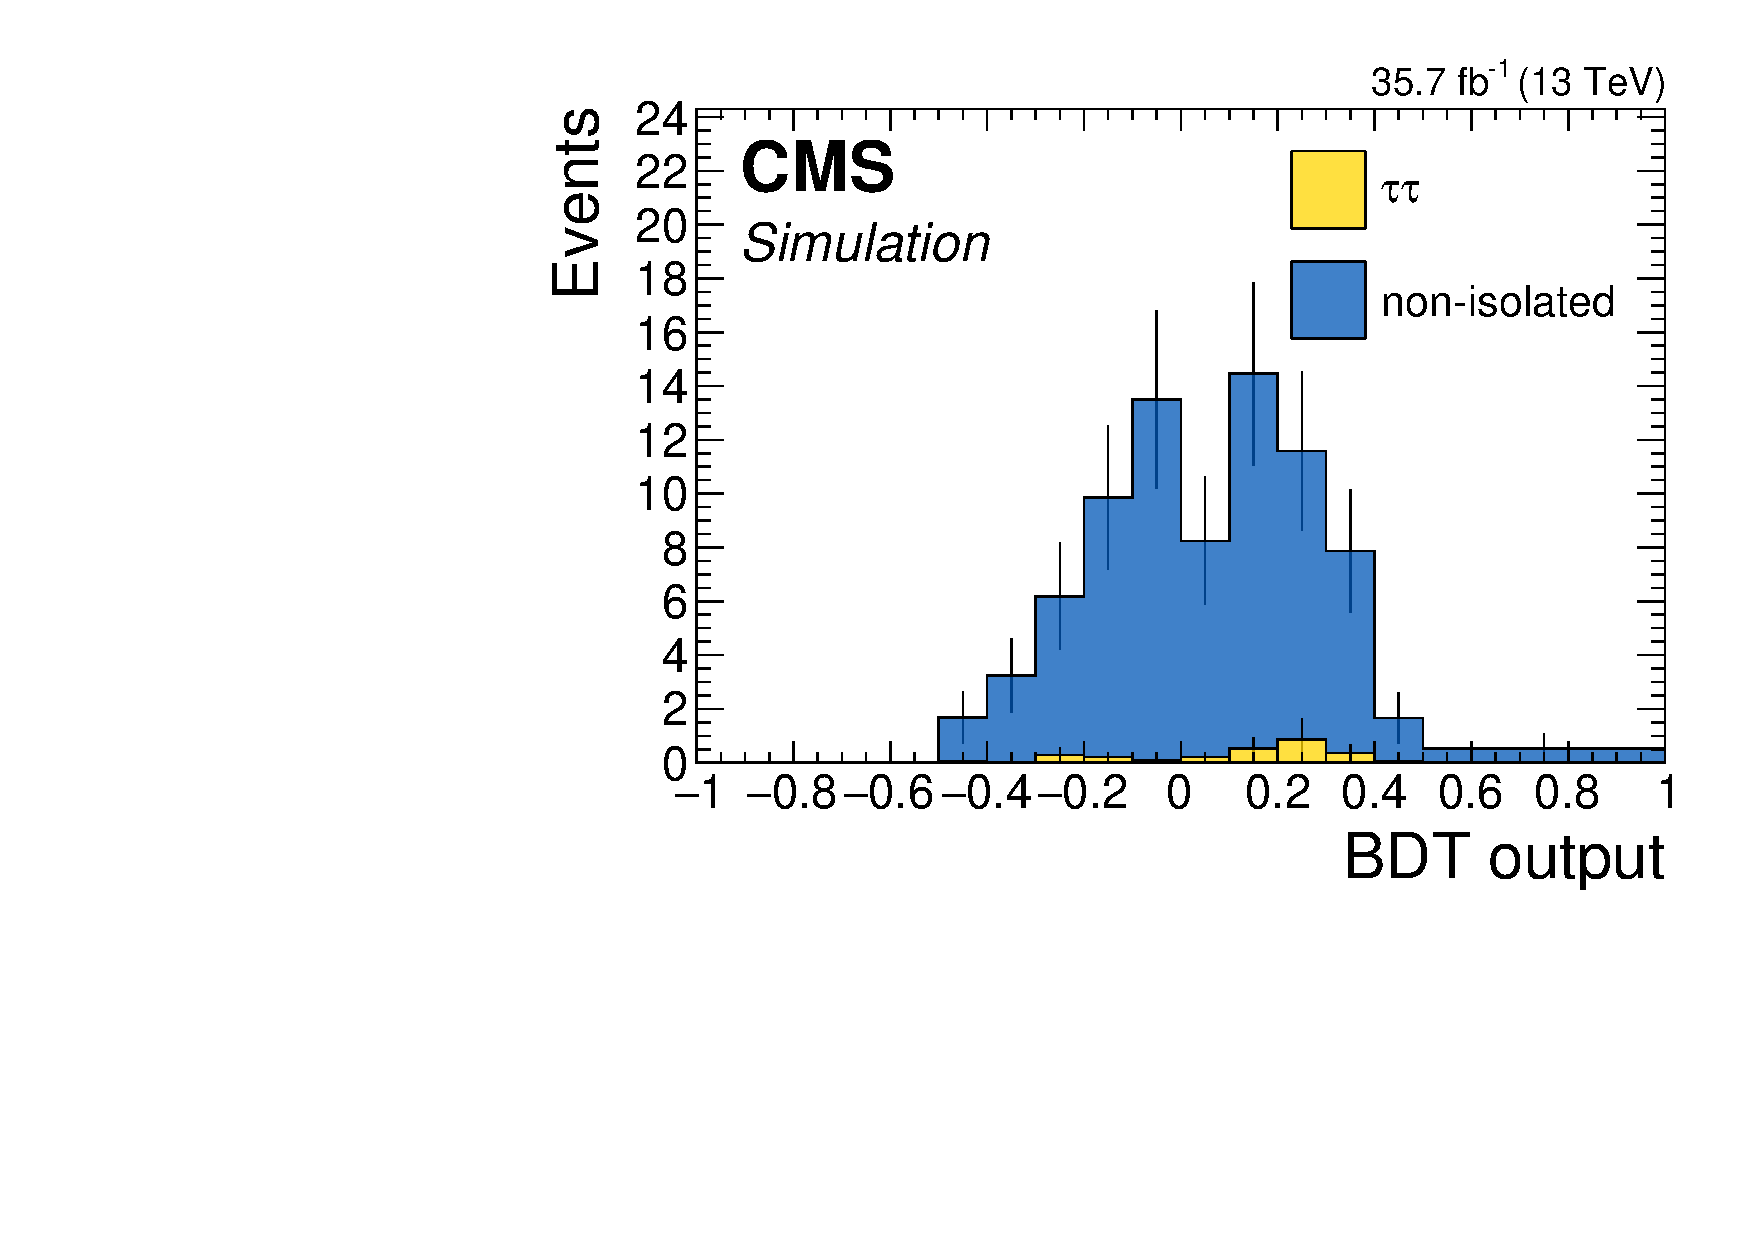
\includegraphics[width=0.48\linewidth]{plots/dimuon_background_estimation_non_isolated_and_tautau_2016/orth-notautau1_newestestest_bin_dilepBDTphase1CorrJetNoMultIso10Dr0.6.pdf} 
 \\
 
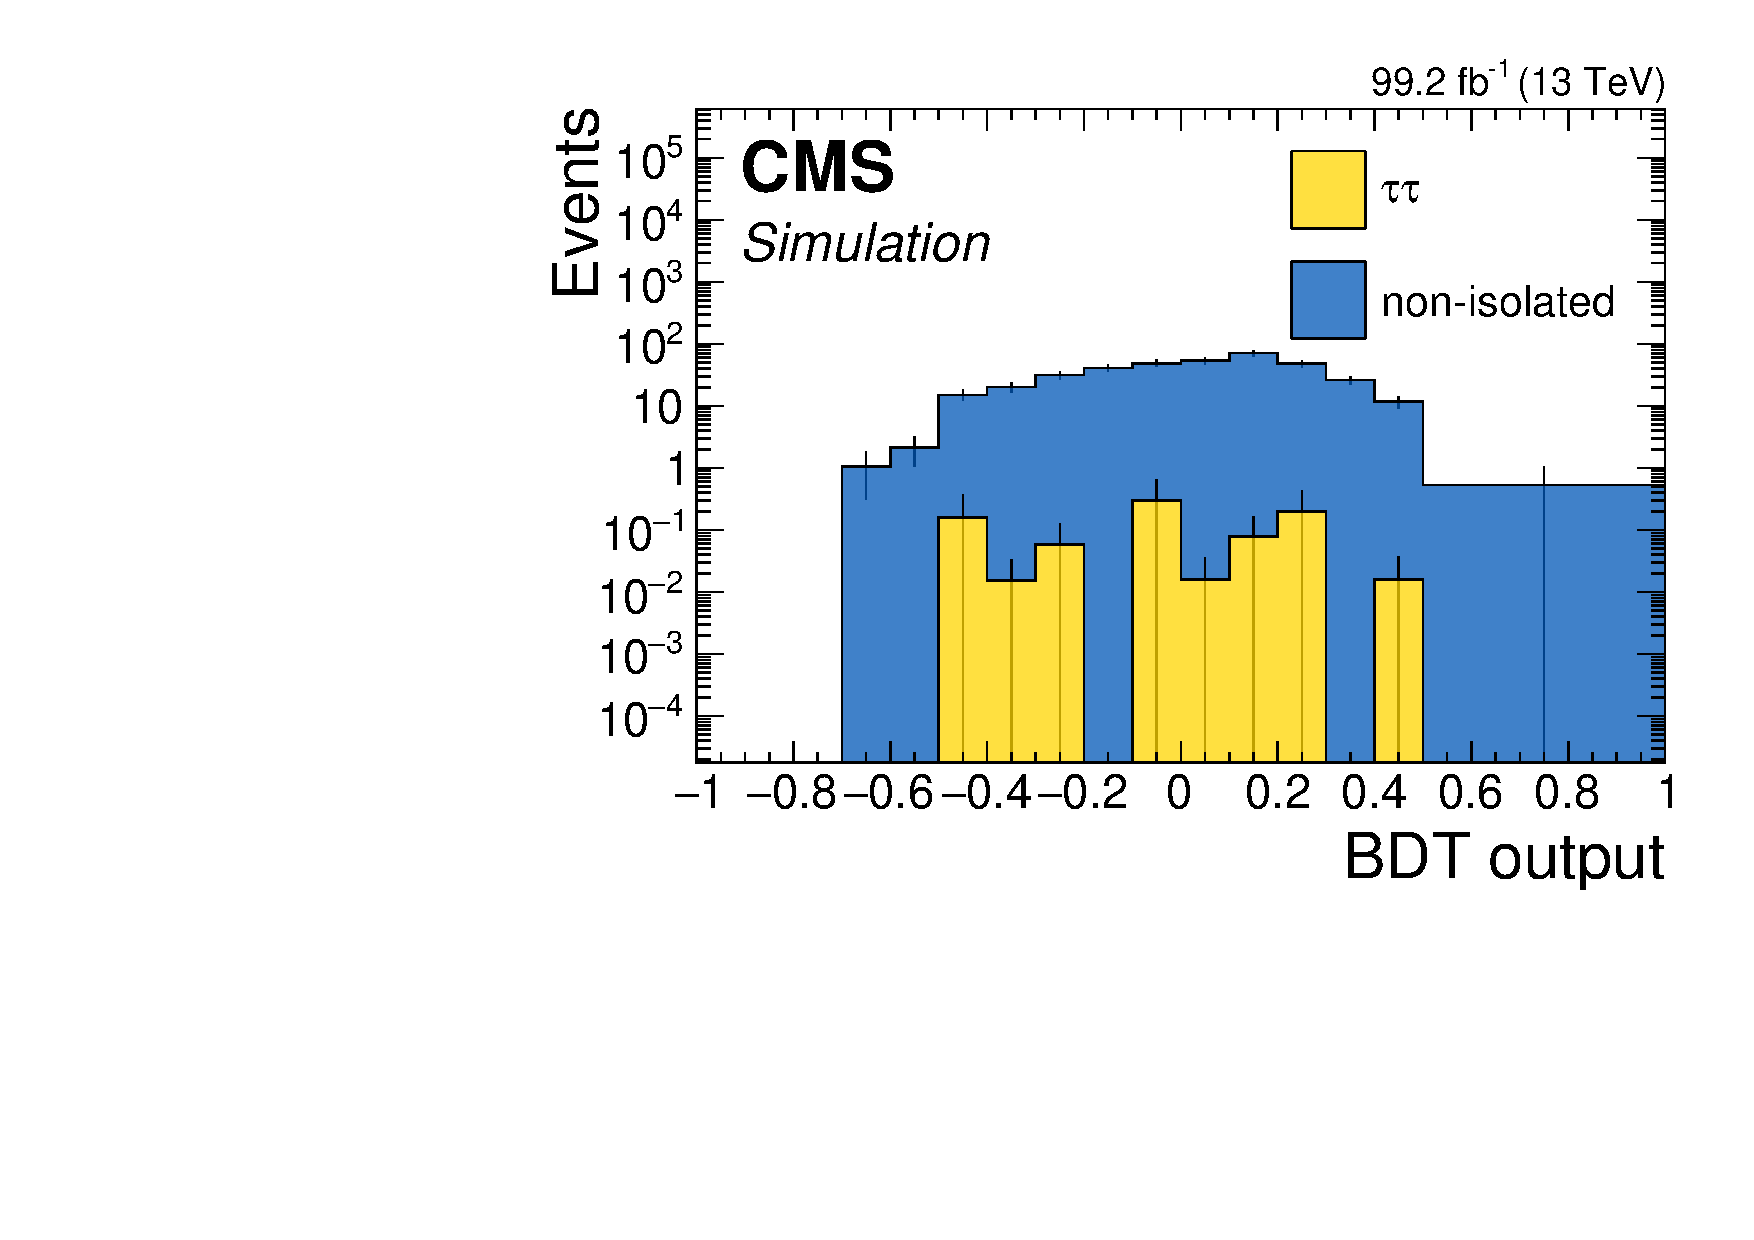
\includegraphics[width=0.48\linewidth]{plots/dimuon_background_estimation_non_isolated_and_tautau_phase1/orth-notautau1_newestestest_bin_dilepBDTphase1CorrJetNoMultIso10Dr0.6_log.pdf} \,
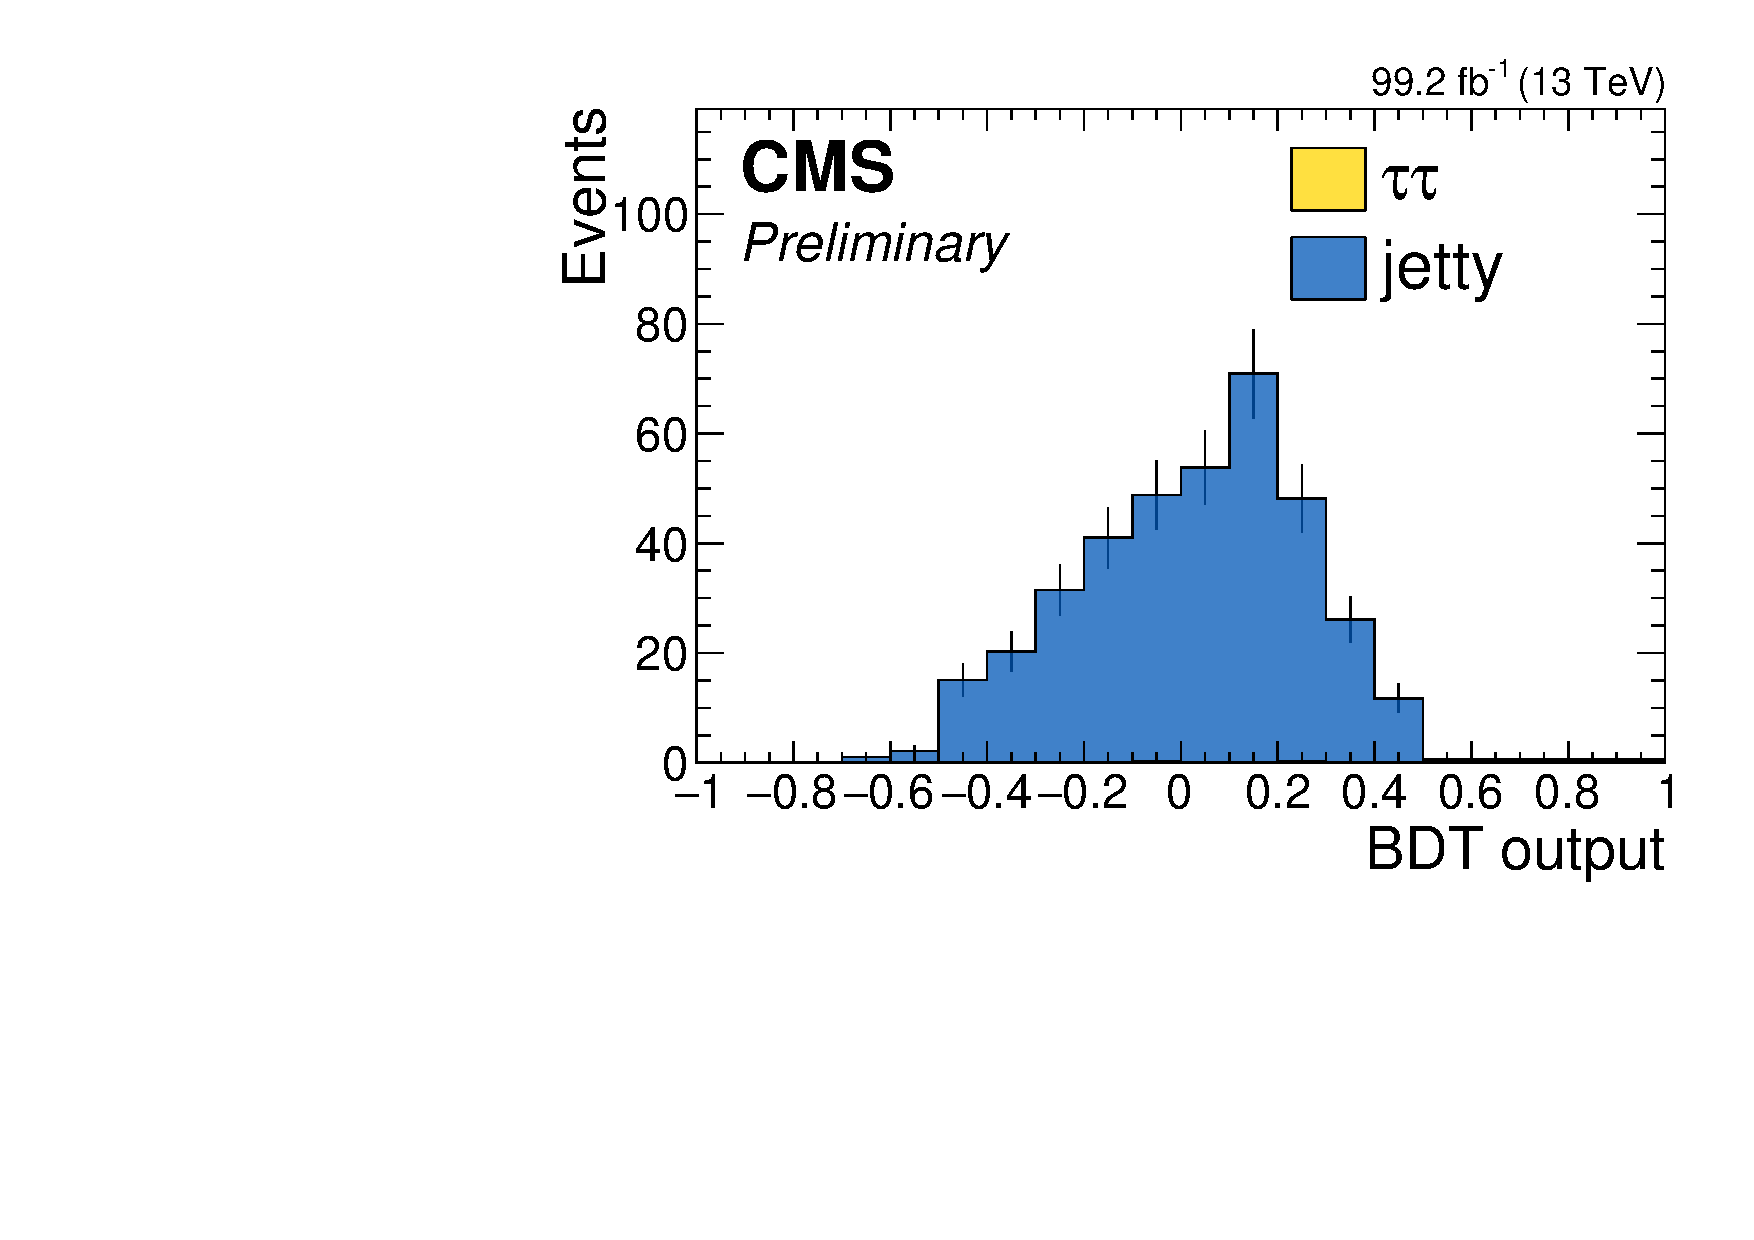
\includegraphics[width=0.48\linewidth]{plots/dimuon_background_estimation_non_isolated_and_tautau_phase1/orth-notautau1_newestestest_bin_dilepBDTphase1CorrJetNoMultIso10Dr0.6.pdf} 
 \\


\caption[Dimuon full background prediction for both phases]{Dimuon full background prediction for phase 0 (top) and phase 1 (bottom) both in log scale (left) and linear scale (right). Blue represents the data-driven jetty non-isolated background, while yellow is the $\tautau$ background.}
\label{fig:data-driven-full-background-prediction}
\end{figure}